~ Begin SubFigureRow { vertical-align: bottom }
~ SubFigure { #fig-subfig1; caption:"Structured discretization" }

~~ Snippet
%--------------------------------------------------------------------------------------------------------------------
% Left lower picture: Structured grid
%--------------------------------------------------------------------------------------------------------------------

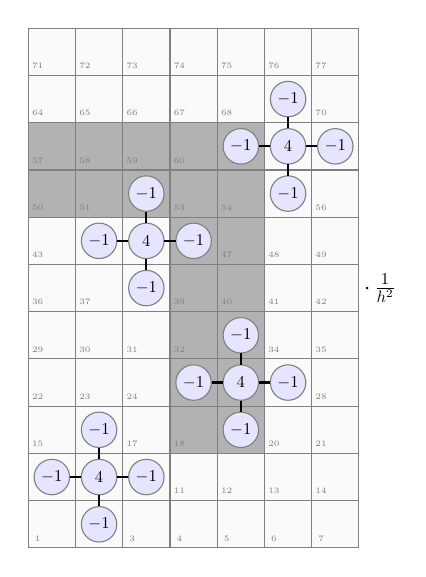
\begin{tikzpicture}
[
 scale=0.6,
 every node/.style ={scale=0.6},
 inner sep=0.5mm,
 BLUECIRC/.style={circle, draw=black!50, fill=blue!10, thin, minimum size=7.5mm},
 REDCIRC/.style={circle, draw=black!50, fill=red!10, thin, minimum size=7.5mm},
 OBST/.style={rectangle, draw=black!50, fill=black!30, thin, minimum size=10mm},
 CELL/.style={rectangle, draw=black!50, fill=black!02,   thin, minimum size=10mm},
 ],
%
\foreach \y in {-1,0,1,2,3,4,5,6,7,8,9}
   \foreach \x in {1,2,3,4,5,6,7}
      {
        \node [CELL]    at ( \x, \y)  {};
       }
 %      
\foreach \y in {1,2,3,4,5,6,7}
   \foreach \x in {4,5}
      {
        \node [OBST]    at ( \x, \y)  {};
       }
%
\foreach \y in {6,7}
   \foreach \x in {1,2,3,4,5}
      {
        \node [OBST]    at ( \x, \y)  {};
       }
\node  at (7.9,4)  {\Large \,$\cdot \,\frac{1}{h^2}$};       
%
\node [BLUECIRC]  (WS)   at ( 2, -1)  {$-1$};
\node [BLUECIRC]  (WW)  at ( 1, 0)  {$-1$};
\node [BLUECIRC]  (WC)   at ( 2, 0)  {$4$};
\node [BLUECIRC]  (WN)   at ( 2, 1)  {$-1$};
\node [BLUECIRC]  (WE)   at ( 3, 0)  {$-1$};
%
\node [BLUECIRC]  (XS)   at ( 5, 1)  {$-1$};
\node [BLUECIRC]  (XW)  at ( 4, 2)  {$-1$};
\node [BLUECIRC]  (XC)   at ( 5, 2)  {$4$};
\node [BLUECIRC]  (XN)   at ( 5, 3)  {$-1$};
\node [BLUECIRC]  (XE)   at ( 6, 2)  {$-1$};
%
\node [BLUECIRC]  (YS)   at ( 3, 4)  {$-1$};
\node [BLUECIRC]  (YW)  at ( 2, 5)  {$-1$};
\node [BLUECIRC]  (YC)   at ( 3, 5)  {$4$};
\node [BLUECIRC]  (YN)   at ( 3, 6)  {$-1$};
\node [BLUECIRC]  (YE)   at ( 4, 5)  {$-1$};
%
\node [BLUECIRC]  (ZS)   at ( 6, 6)  {$-1$};
\node [BLUECIRC]  (ZW)  at ( 5, 7)  {$-1$};
\node [BLUECIRC]  (ZC)   at ( 6, 7)  {$4$};
\node [BLUECIRC]  (ZN)   at ( 6, 8)  {$-1$};
\node [BLUECIRC]  (ZE)   at ( 7, 7)  {$-1$};
%
\draw [thick]  (WC.south)  -- (WS.north) ;
\draw [thick]  (WC.west)   -- (WW.east) ;
\draw [thick]  (WC.north)  -- (WN.south) ;
\draw [thick]  (WC.east)  -- (WE.west) ;
%
\draw [thick]  (XC.south)  -- (XS.north) ;
\draw [thick]  (XC.west)   -- (XW.east) ;
\draw [thick]  (XC.north)  -- (XN.south) ;
\draw [thick]  (XC.east)  -- (XE.west) ;
%
\draw [thick]  (YC.south)  -- (YS.north) ;
\draw [thick]  (YC.west)   -- (YW.east) ;
\draw [thick]  (YC.north)  -- (YN.south) ;
\draw [thick]  (YC.east)  -- (YE.west) ;
%
\draw [thick]  (ZC.south)  -- (ZS.north) ;
\draw [thick]  (ZC.west)   -- (ZW.east) ;
\draw [thick]  (ZC.north)  -- (ZN.south) ;
\draw [thick]  (ZC.east)  -- (ZE.west) ;
%
\draw[color=gray]   node at (0.7,-1.3) {\tiny 1};
\draw[color=gray]   node at (2.7,-1.3) {\tiny 3};
\draw[color=gray]   node at (3.7,-1.3) {\tiny 4};
\draw[color=gray]   node at (4.7,-1.3) {\tiny 5};
\draw[color=gray]   node at (5.7,-1.3) {\tiny 6};
\draw[color=gray]   node at (6.7,-1.3) {\tiny 7};
\draw[color=gray]   node at (3.7,-0.3) {\tiny 11};
\draw[color=gray]   node at (4.7,-0.3) {\tiny 12};
\draw[color=gray]   node at (5.7,-0.3) {\tiny 13};
\draw[color=gray]   node at (6.7,-0.3) {\tiny 14};
\draw[color=gray]   node at (0.7,0.7) {\tiny 15};
\draw[color=gray]   node at (2.7,0.7) {\tiny 17};
\draw[color=gray]   node at (3.7,0.7) {\tiny 18};
\draw[color=gray]   node at (5.7,0.7) {\tiny 20};
\draw[color=gray]   node at (6.7,0.7) {\tiny 21};
\draw[color=gray]   node at (0.7,1.7) {\tiny 22};
\draw[color=gray]   node at (1.7,1.7) {\tiny 23};
\draw[color=gray]   node at (2.7,1.7) {\tiny 24};
\draw[color=gray]   node at (6.7,1.7) {\tiny 28};
\draw[color=gray]   node at (0.7,2.7) {\tiny 29};
\draw[color=gray]   node at (1.7,2.7) {\tiny 30};
\draw[color=gray]   node at (2.7,2.7) {\tiny 31};
\draw[color=gray]   node at (3.7,2.7) {\tiny 32};
\draw[color=gray]   node at (5.7,2.7) {\tiny 34};
\draw[color=gray]   node at (6.7,2.7) {\tiny 35};
\draw[color=gray]   node at (0.7,3.7) {\tiny 36};
\draw[color=gray]   node at (1.7,3.7) {\tiny 37};
\draw[color=gray]   node at (3.7,3.7) {\tiny 39};
\draw[color=gray]   node at (4.7,3.7) {\tiny 40};
\draw[color=gray]   node at (5.7,3.7) {\tiny 41};
\draw[color=gray]   node at (6.7,3.7) {\tiny 42};
\draw[color=gray]   node at (0.7,4.7) {\tiny 43};
\draw[color=gray]   node at (4.7,4.7) {\tiny 47};
\draw[color=gray]   node at (5.7,4.7) {\tiny 48};
\draw[color=gray]   node at (6.7,4.7) {\tiny 49};
\draw[color=gray]   node at (0.7,5.7) {\tiny 50};
\draw[color=gray]   node at (1.7,5.7) {\tiny 51};
\draw[color=gray]   node at (3.7,5.7) {\tiny 53};
\draw[color=gray]   node at (4.7,5.7) {\tiny 54};
\draw[color=gray]   node at (6.7,5.7) {\tiny 56};
\draw[color=gray]   node at (0.7,6.7) {\tiny 57};
\draw[color=gray]   node at (1.7,6.7) {\tiny 58};
\draw[color=gray]   node at (2.7,6.7) {\tiny 59};
\draw[color=gray]   node at (3.7,6.7) {\tiny 60};
\draw[color=gray]   node at (0.7,7.7) {\tiny 64};
\draw[color=gray]   node at (1.7,7.7) {\tiny 65};
\draw[color=gray]   node at (2.7,7.7) {\tiny 66};
\draw[color=gray]   node at (3.7,7.7) {\tiny 67};
\draw[color=gray]   node at (4.7,7.7) {\tiny 68};
\draw[color=gray]   node at (6.7,7.7) {\tiny 70};
\draw[color=gray]   node at (0.7,8.7) {\tiny 71};
\draw[color=gray]   node at (1.7,8.7) {\tiny 72};
\draw[color=gray]   node at (2.7,8.7) {\tiny 73};
\draw[color=gray]   node at (3.7,8.7) {\tiny 74};
\draw[color=gray]   node at (4.7,8.7) {\tiny 75};
\draw[color=gray]   node at (5.7,8.7) {\tiny 76};
\draw[color=gray]   node at (6.7,8.7) {\tiny 77};
%
\end{tikzpicture}
~~
~
~ SubFigure { #fig-subfig1; caption:"Unstructured discretization" }
~~ Snippet
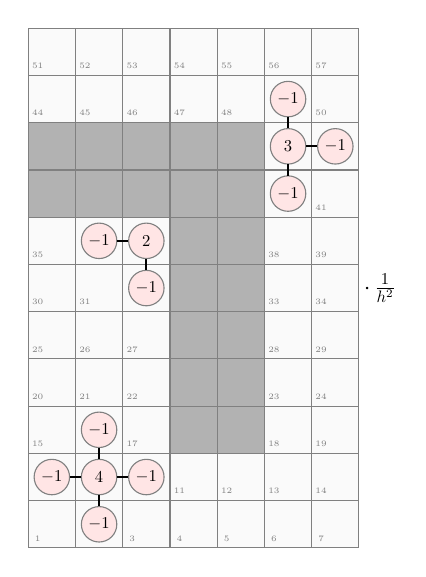
\begin{tikzpicture}
[
 scale=0.6,
 every node/.style ={scale=0.6},
 inner sep=0.5mm,
 BLUECIRC/.style={circle, draw=black!50, fill=blue!10,  thin, minimum size=7.5mm},
 REDCIRC/.style={circle, draw=black!50, fill=red!10, thin, minimum size=7.5mm},
 OBST/.style={rectangle, draw=black!50, fill=black!30, thin, minimum size=10mm},
 CELL/.style={rectangle, draw=black!50, fill=black!02,   thin, minimum size=10mm},
 ],
%
\foreach \y in {-1,0,1,2,3,4,5,6,7,8,9}
   \foreach \x in {1,2,3,4,5,6,7}
      {
        \node [CELL]    at ( \x, \y)  {};
       }
 %      
\foreach \y in {1,2,3,4,5,6,7}
   \foreach \x in {4,5}
      {
        \node [OBST]    at ( \x, \y)  {};
       }
%
\foreach \y in {6,7}
   \foreach \x in {1,2,3,4,5}
      {
        \node [OBST]    at ( \x, \y)  {};
       }
\node    at ( 7.9, 4)  {\Large \,$\cdot \,\frac{1}{h^2}$};
%
\node [REDCIRC]  (WS)   at ( 2, -1)  {$-1$};
\node [REDCIRC]  (WW)  at ( 1, 0)  {$-1$};
\node [REDCIRC]  (WC)   at ( 2, 0)  {$4$};
\node [REDCIRC]  (WN)   at ( 2, 1)  {$-1$};
\node [REDCIRC]  (WE)   at ( 3, 0)  {$-1$};
%
\node [REDCIRC]  (XS)   at ( 6, 6)  {$-1$};
\node [REDCIRC]  (XC)   at ( 6, 7)  {$3$};
\node [REDCIRC]  (XN)   at ( 6, 8)  {$-1$};
\node [REDCIRC]  (XE)   at ( 7, 7)  {$-1$};
%
\node [REDCIRC]  (YS)   at ( 3, 4)  {$-1$};
\node [REDCIRC]  (YW)  at ( 2, 5)  {$-1$};
\node [REDCIRC]  (YC)   at ( 3, 5)  {$2$};
%
\draw [thick]  (WC.south)  -- (WS.north) ;
\draw [thick]  (WC.west)   -- (WW.east) ;
\draw [thick]  (WC.north)  -- (WN.south) ;
\draw [thick]  (WC.east)  -- (WE.west) ;
%
\draw [thick]  (XC.south)  -- (XS.north) ;
\draw [thick]  (XC.north)  -- (XN.south) ;
\draw [thick]  (XC.east)  -- (XE.west) ;
%
\draw [thick]  (YC.south)  -- (YS.north) ;
\draw [thick]  (YC.west)   -- (YW.east) ;
%
%
\draw[color=gray]   node at (0.7,-1.3) {\tiny 1};
\draw[color=gray]   node at (2.7,-1.3) {\tiny 3};
\draw[color=gray]   node at (3.7,-1.3) {\tiny 4};
\draw[color=gray]   node at (4.7,-1.3) {\tiny 5};
\draw[color=gray]   node at (5.7,-1.3) {\tiny 6};
\draw[color=gray]   node at (6.7,-1.3) {\tiny 7};
\draw[color=gray]   node at (3.7,-0.3) {\tiny 11};
\draw[color=gray]   node at (4.7,-0.3) {\tiny 12};
\draw[color=gray]   node at (5.7,-0.3) {\tiny 13};
\draw[color=gray]   node at (6.7,-0.3) {\tiny 14};
\draw[color=gray]   node at (0.7,0.7) {\tiny 15};
\draw[color=gray]   node at (2.7,0.7) {\tiny 17};
\draw[color=gray]   node at (5.7,0.7) {\tiny 18};
\draw[color=gray]   node at (6.7,0.7) {\tiny 19};
\draw[color=gray]   node at (0.7,1.7) {\tiny 20};
\draw[color=gray]   node at (1.7,1.7) {\tiny 21};
\draw[color=gray]   node at (2.7,1.7) {\tiny 22};
\draw[color=gray]   node at (5.7,1.7) {\tiny 23};
\draw[color=gray]   node at (6.7,1.7) {\tiny 24};
\draw[color=gray]   node at (0.7,2.7) {\tiny 25};
\draw[color=gray]   node at (1.7,2.7) {\tiny 26};
\draw[color=gray]   node at (2.7,2.7) {\tiny 27};
\draw[color=gray]   node at (5.7,2.7) {\tiny 28};
\draw[color=gray]   node at (6.7,2.7) {\tiny 29};
\draw[color=gray]   node at (0.7,3.7) {\tiny 30};
\draw[color=gray]   node at (1.7,3.7) {\tiny 31};
\draw[color=gray]   node at (5.7,3.7) {\tiny 33};
\draw[color=gray]   node at (6.7,3.7) {\tiny 34};
\draw[color=gray]   node at (0.7,4.7) {\tiny 35};
\draw[color=gray]   node at (5.7,4.7) {\tiny 38};
\draw[color=gray]   node at (6.7,4.7) {\tiny 39};
\draw[color=gray]   node at (6.7,5.7) {\tiny 41};
\draw[color=gray]   node at (0.7,7.7) {\tiny 44};
\draw[color=gray]   node at (1.7,7.7) {\tiny 45};
\draw[color=gray]   node at (2.7,7.7) {\tiny 46};
\draw[color=gray]   node at (3.7,7.7) {\tiny 47};
\draw[color=gray]   node at (4.7,7.7) {\tiny 48};
\draw[color=gray]   node at (6.7,7.7) {\tiny 50};
\draw[color=gray]   node at (0.7,8.7) {\tiny 51};
\draw[color=gray]   node at (1.7,8.7) {\tiny 52};
\draw[color=gray]   node at (2.7,8.7) {\tiny 53};
\draw[color=gray]   node at (3.7,8.7) {\tiny 54};
\draw[color=gray]   node at (4.7,8.7) {\tiny 55};
\draw[color=gray]   node at (5.7,8.7) {\tiny 56};
\draw[color=gray]   node at (6.7,8.7) {\tiny 57};
\end{tikzpicture}
%
~~
~
~ End SubFigureRow

